\documentclass[12pt, twoside]{article}
\usepackage{jmlda}
\usepackage[]{algorithmic}
\usepackage{graphicx}
\usepackage{multicol}
\usepackage{caption}
\usepackage{subfig}

\usepackage[russian]{babel}

%images
\usepackage{graphicx}
\graphicspath{ {./images/} 

%hyperlinks
\usepackage{hyperref}
\hypersetup{
    colorlinks=true,
    linkcolor=blue,
    filecolor=magenta,      
    urlcolor=cyan,
    pdftitle={Overleaf Example},
    pdfpagemode=FullScreen,
    }


% Compatibility for biblatex
\usepackage{csquotes}

% Load biblatex before cleveref
\usepackage[backend=bibtex]{biblatex}
\addbibresource{references.bib}


\newcommand{\hdir}{.}
\newtheorem{statement}{Утверждение}

\newcommand{\bz}{\mathbf{z}}
\newcommand{\bx}{\mathbf{x}}
\newcommand{\by}{\mathbf{y}}
\newcommand{\bv}{\mathbf{v}}
\newcommand{\bw}{\mathbf{w}}
\newcommand{\ba}{\mathbf{a}}
\newcommand{\bb}{\mathbf{b}}
\newcommand{\bp}{\mathbf{p}}
\newcommand{\bq}{\mathbf{q}}
\newcommand{\bt}{\mathbf{t}}
\newcommand{\bu}{\mathbf{u}}
\newcommand{\bT}{\mathbf{T}}
\newcommand{\bX}{\mathbf{X}}
\newcommand{\bZ}{\mathbf{Z}}
\newcommand{\bS}{\mathbf{S}}
\newcommand{\bH}{\mathbf{H}}
\newcommand{\bW}{\mathbf{W}}
\newcommand{\bY}{\mathbf{Y}}
\newcommand{\bU}{\mathbf{U}}
\newcommand{\bQ}{\mathbf{Q}}
\newcommand{\bP}{\mathbf{P}}
\newcommand{\bA}{\mathbf{A}}
\newcommand{\bB}{\mathbf{B}}
\newcommand{\bC}{\mathbf{C}}
\newcommand{\bE}{\mathbf{E}}
\newcommand{\bF}{\mathbf{F}}
\newcommand{\bomega}{\boldsymbol{\omega}}
\newcommand{\bOmega}{\boldsymbol{\Omega}}
\newcommand{\btheta}{\boldsymbol{\theta}}
\newcommand{\bTheta}{\boldsymbol{\Theta}}
\newcommand{\bgamma}{\boldsymbol{\gamma}}
\newcommand{\bdelta}{\boldsymbol{\delta}}
\newcommand{\bDelta}{\boldsymbol{\Delta}}
\newcommand{\bPsi}{\boldsymbol{\Psi}}
\newcommand{\bpsi}{\boldsymbol{\psi}}
\newcommand{\bxi}{\boldsymbol{\xi}}
\newcommand{\bchi}{\boldsymbol{\chi}}
\newcommand{\bzeta}{\boldsymbol{\zeta}}
\newcommand{\blambda}{\boldsymbol{\lambda}}
\newcommand{\beps}{\boldsymbol{\varepsilon}}
\newcommand{\bZeta}{\boldsymbol{Z}}
% mathcal
\newcommand{\cX}{\mathcal{X}}
\newcommand{\cY}{\mathcal{Y}}
\newcommand{\cW}{\mathcal{W}}
\newcommand{\cF}{\mathcal{F}}

\newcommand{\HH}{\mathbb{H}}
\newcommand{\RR}{\mathbb{R}}
\newcommand{\EE}{\mathbb{E}}
% transpose
\newcommand{\T}{^{\mathsf{T}}}
\newcommand{\argmax}{\mathop{\mathrm{argmax}}}
\newcommand{\argmin}{\mathop{\mathrm{argmin}}}

% method name
% \newcommand{\mname}{LoSPIN}



\begin{document}

\title
    [] % краткое название; не нужно, если полное название влезает в~колонтитул
    {Low-rank self-play fine-tuning for small LLMs}
\author
    [] % список авторов (не более трех) для колонтитула; не нужен, если основной список влезает в колонтитул
    {П.\,Ю.~Мун, Н.\,В.~Охотников, А.\,В.~Грабовой} % основной список авторов, выводимый в оглавление
    [П.\,Ю.~Мун$^1$, Н.\,В.~Охотников$^2$, А.\,В.~Грабовой$^3$] % список авторов, выводимый в заголовок; не нужен, если он не отличается от основного
%\email
%   {anton39reg@mail.ru; anton.khritankov@phystech.edu}

%\thanks
%    {Работа выполнена при
%     %частичной
%     финансовой поддержке РФФИ, проекты \No\ \No 00-00-00000 и 00-00-00001.}
%\organization
%    {$^1$Организация, адрес; $^2$Организация, адрес}
\abstract
  {В работе исследуется проблема дообучения больших языковых моделей (LLM) в условиях ограниченных ресурсов. Под ограниченными ресурсами понимается видеопамять, человеческое участие и время обучения. В работе рассматриваются модели до 1.5B. Предлагается метод дообучения, основанный на внедрении адаптеров LoRA, малоранговых раложений матриц, в слои архитектуры трансформера, и использовании стратегии self-play - текущая итерация генерирует предсказания, а обучающаяся повышает качество с помощью разграничения настоящих предсказаний от сгенерированных. Метод может снизить количество обучаемых параметров в 10000, и память в три раза, также он не требует размеченных данных помимо используемых на этапе SFT. Для анализа качества метода будет использована группа датасетов, таких как MMLU, Winogrande.


\bigskip
\noindent
\textbf{Ключевые слова}: \emph {LLM, LoRA, selp-play, SFT}
}
%данные поля заполняются редакцией журнала
\doi{}
\receivedRus{}
\receivedEng{}

\maketitle
\linenumbers
\section{Введение}
Большие языковые модели (LLM) демонстрируют исключительные возможности в широком спектре областей, которые могут требовать специализированных знаний. Примерами таких областей могут служить: программирование \parencite{Chen2021}, генерация текстов \parencite{Touvron2023}, обращения к базам данных \parencite{Zhong2017}. Обычно процесс обучения LLM состоит из нескольких этапов: предварительного обучения, и этапов дообучения: SFT, обучение на предварительно размеченном наборе данных, и RLHF, во время которого необходим эксперт-человек, оценивающий ответы модели. Предварительное обучение требует огромных вычислительных ресурсов, поэтому часто используют публичные предобученные модели (Llama3 \parencite{Dubey2024}, Qwen2.5 \parencite{Yang2025}) и настраивают под целевую задачу. Но также проблема ограниченности ресурсов встречается и на этапах дообучения SFT и RLHF. Ограниченность ресурсов проявляется в недостатке видеопамяти для хранения и обновления параметров модели, необходимости в размеченных данных для повышения качества и времени обучения.

В работе исследуются методы повышения эффективности обучения моделей в условиях ограниченных ресурсов. В частности прдлагается метод дообучения LLM, который значительно снижает потребление видеопамяти, а также убирает необходимость в прямом человеческом участии. Метод основан на двух идеях. 

\begin{itemize}
  \item Во-первых, внедрение адаптеров LoRA в слои трансформера. Предполагается сравнительно маленькая внутренняя размерность пространства параметров, и рассматриваемый метод снижает размерность пространства параметров. 
  
  \vspace{8}
   
  \item Во-вторых, механизме self-play для обучения адаптеров. Механизм состоит из последовательных игр модели со своей предыдущей версией. Предыдущая версия генерирует ответы по промптам части датасета на этапе SFT, а модель пытается различить настоящий ответ от сгенерированного. Общий метод исследуется в статье \parencite{Chen2024a}, а  в данной работе он применяется исключительно к адаптерам LoRA. 
\end{itemize}

Предложенный метод развивается в двух направлениях: снижение требований к видео памяти и снижение человеческого участия. В обоих направлениях есть близкие альтернативы:

\begin{itemize}
  \item Многие существующие решения по снижению требуемой памяти также применяют адаптеры LoRA с использованием других интсрументов. Одним из лучших методов является QLoRA \parencite{Dettmers2023}, который предлагает 4х битные float и квантизацию, значительно снижая необходимую память. В отличии от LoRA, которая снижает количество обучаемых параметров, QLoRA также уменьшает размер параметров модели с помощью 4х битных NormalFloat, что приводит в меньшим требованиям к видеопамяти. С другой стороны, QLoRA требует передового оборудования для применения, что может являться существенным ограниченим в условиях нехватки ресурсов. 

  \vspace{8}
  
  \item В направлении снижения человеческого участия можно выделить методы оптимизирующие этап RLHF. Одним из таких являетя метод DPO \parencite{Rafailov2023a}, который снижает зависимость от человеского оценивания результата. В то же время предложенный метод не требует размеченных данных, помимо тех, что используются на SFT.
\end{itemize}

Конечной целью работы является исследование оправданности применения предложенного метода к маленьким LLM в условиях ограниченных ресурсов.

\vspace{10}

\section{Связанные работы}

TODO:

\vspace{10}

\section{Постановка задачи}

Будем обозначать за $\bTheta$ - пространство всевозможных параметров трансформера, $p_{\btheta}$ - модель , а $\btheta \in \bTheta$ -  ее параметры. В задаче ставится ограничение на количество параметров модели, то есть $\|\bTheta\| \le \mathbf{K}$. Также используются последовательности $\bx = [x_1, ..., x_n]$, $\by' = [y_1', ..., y_m']$ и $\by=[y_1, ..., y_m]$, которые интерепретируются как промпт, ответ модели, истинный ответ соостветсвенно. Изначально $\btheta = \btheta_0$, где $\btheta_0 \in \bTheta$, на каждом шаге метода параметры модели будут обновляться, $\btheta_t$ - параметры на шаге t.

Также для дальнейшей работы с методом введем вероятностные предположения о распределениях данных: $\bx \sim q(\cdot)$,  $\by \sim p_{data}(\cdot | \bx)$. 

Теперь перейдем к введению понятий для обозначений методов.

\paragraph{Адаптеры LoRA}
Адаптер LoRA представлен произведением двух матриц $A \cdot B$ и может быть встроен в любую обучаемую матрицу весов $W_0$. Во время дообучения матрица весов $W_0$ заморожена, то есть не меняется, и обучаются только матрицы $A$ и $B$, что может помочь снизить количество обучаемых параметров и соответственно требуемую память для дообучения. В конце модель модель использует сумму изначальной матрицы с адаптером, $W = W_0 + A \cdot B$.

В данной работе адаптеры LoRA встраиваются на всех слоях в матрицы: $W_q, W_k, W_v$ - query/key/value матрицы блоков self-attention в архитектуре трансформера. Обозначим значения всех встраиваемых параметров на шаге t за $\bDelta\btheta_t$, тогда

$$\btheta_t = \btheta_0 + \bDelta\btheta_t$$

\paragraph{Подробное описание SPIN}

В центре механизма self-play находится игра между: моделью игроком и моделью противником. Цель противника сгенерировать ответы, которые были бы неразличимы с настоящими ответами, а цель игрока уметь различать настоящие ответы от сгенерированных. В рамках дообучения противником является прошлая итерация модели, а игроком текущая итерация, которая обучается.

Рассмотрим итерацию t+1, противником на данной итерации является $p_{\btheta_t}$, которая по промптам $\bx$ генерирует ответы $\by'$, а игроком $p_{\btheta_{t+1}}$. Метод состоит из двух шагов: обучение игрока, обновление противника

\begin{itemize}
    \item В качестве целевой функции для первого шага используется:
    \begin{align}
        f_{t+1} &= \argmax_{f \in \cF_{t}}\EE_{\bx\sim q(\cdot), \by\sim p_{data}(\cdot | \bx)}\big[l(f(\bx, \by) - f(\bx, \by')) \big], \label{eq:f*1}
    \end{align}
    , где $l = log(1 + exp(-t))$, а $\cF_t$ - некоторое семейство функций.

    \vspace{8}

    \item Для обновления противника используется следующая функция:
    
    \begin{align} 
        p_{\btheta_{t+1}} = \argmax_ {p}\EE_{\bx \sim q(\cdot), \by\sim p(\cdot|\bx)} [f_{t+1}(\bx, \by)] - \lambda \EE_{\bx\sim q(\cdot)}\mathrm{KL}\big(p(\cdot|\bx)||p_{\btheta_t}(\cdot|\bx)\big), \phantomsection\label{eq:update}
    \end{align} 
    
    , где $\lambda$ - коэффициент регуляризации похожести итераций, а $KL$ - дивергенция Кульбака-Лейблера. Регуляризация добавлена с целью контроля обучаемой итерации, чтобы $p_\btheta_{t+1}$  не сильно отличалась от $p_\btheta_t$
    
    
\end{itemize}

\paragraph{Одношаговое описание SPIN}

Примечательно, что последнее выражение \eqref{eq:update} на $p_{\btheta_{t+1}}$ имеет аналитическое решение $\hat p_{\btheta_{t+1}}$:

\begin{align}
\hat{p}_{\btheta_{t+1}}(\by|\bx) \propto p_{\btheta_t}(\by|\bx) \exp\big(\lambda^{-1}f_{t+1}(\bx, \by)\big). \label{eq:closed form solution}  
\end{align}

Важно упомянуть, что у такого аналитического решения может не быть представления в виде функции, параметризованной элементами из $\bTheta$, то есть $\hat{p}_{\btheta_{t+1}}$ не обязательно принадлежит семейству $\{p_{\btheta} | \btheta \in \bTheta\}$. Тогда рассмотрим класс функций для $f_{t+1}$:

\begin{align}
\cF_{t} = \bigg\{\lambda\cdot \log \frac{p_{\btheta}(\by | \bx)}{p_{\mathrm{\btheta_t}}(\by | \bx)}\bigg|\btheta \in \bTheta\bigg\},   \label{eq:function class0} 
\end{align}

Подставляя элементы полученного семейства в формулу 1, получим искомый критерий качеста, используемый при обучении.

\begin{align}
L_{SPIN}= \EE_{\bx\sim q(\cdot), \by\sim p_{data}(\cdot | \bx)}\bigg[\ell\bigg(\lambda \log \frac{p_{\btheta}(\by | \bx)}{p_{\btheta_t}(\by | \bx)}-\lambda \log \frac{p_{\btheta}(\by' | \bx)}{p_{\btheta_t}(\by' | \bx)}\bigg)\bigg], \label{eq:loss}  
\end{align}

Тогда правило обновление параметров имеет вид:

\begin{align}
    \btheta_{t+1} = \argmin_{\btheta \in \bTheta} L_{SPIN} (\btheta, \btheta_t)
\end{align}


\paragraph{Применение SPIN к адаптерам}

Обозначим за $\bOmega \subset \bTheta$ - подпространство весов адаптеров LoRA в архитектуре трансформера. Заметим, что подставление параметров адаптеров LoRA $\bDelta\btheta$ сужает рассматриваемый класс функций $\{p_{\btheta_0 + \bDelta\btheta} | \bDelta\btheta \in \bOmega\} \subset \{p_{\btheta} | \btheta \in \bTheta\}$, но все равно может быть применим в полученному критерию качества $L_{SPIN}$

\begin{align}
    \bDelta\btheta_{t+1} = \argmin_{\bDelta\btheta \in \bOmega} L_{SPIN} (\btheta_0 + \bDelta\btheta, \btheta_0 + \bDelta \btheta_t)
\end{align}

\section{Вычислительный эксперимент}

Целью данного эксперимента является подтверждение сохранения или повышению качества модели при дообучении предложенным методом. Особое внимание уделяется контролю затрачиваемых ресурсов и измерению времени обучения.

Для начало необходимо задать ограничение $\mathbf{K} = 5\cdot10^8$, отвечающий за ограничение на количество параметров модели $\| \bTheta\| \le \mathbf{K}$. Значение обусловлено используемым оборудованием Tesla T4 из Google Colab, память 16 GB, количество ядер 2560. 

\paragraph{Описание базового эксперимента}
В качестве предобученной модели взята трансформерная модель \href{https://huggingface.co/Qwen/Qwen2.5-0.5B}{qwen2.5-0.5B} для задачи генерации текстов, так как она достигает верхней границы на ограничение по параметрам, а также является новой моделью, показывающей отличный результат на leaderboards.

Обучение происходит на датасете \href{https://huggingface.co/datasets/openai/gsm8k}{GSM8K}, состоящем из более чем 8000 математических задач на простую арифметику: $+, -, \%, \cdot$. Все задачи данного уровня должен быть способен решать ученик средних классов. Ответ представлен в виде рассуждения, использующего математические вычисления.

Во время обучения в матрицы:  $W_q, W_k, W_v$ были встроены адаптеры LoRA и соответственно остальные параметры были заморожены. Обучение происходило на трех эпохах, а размер батча был равен 2.

\paragraph{Результаты}

[Так как особо результатов нет, то будет просто описан результат по единственной обученной модели]

\href{https://github.com/MuQlanyu/2025-Project-178/blob/main/notebooks/reports/report_20.03.ipynb}{Ссылка на код}

Обучение \href{https://huggingface.co/Qwen/Qwen2.5-0.5B}{qwen2.5-0.5B} с ограничением только в 4000 объектов датасета заняло 8955 секунд $\sim 2.5$ часа. В процессе обучения пиковое значение используемой видеопамяти достигало 10.3 GB, причем при запуске модели с размером батча равным 4 пиковое значение используемой памяти превышало максимум. Итоговый лосс на обучающей выборке составил 0.7377.

Далее будет представлен график обучения модели, так как того требует задание.

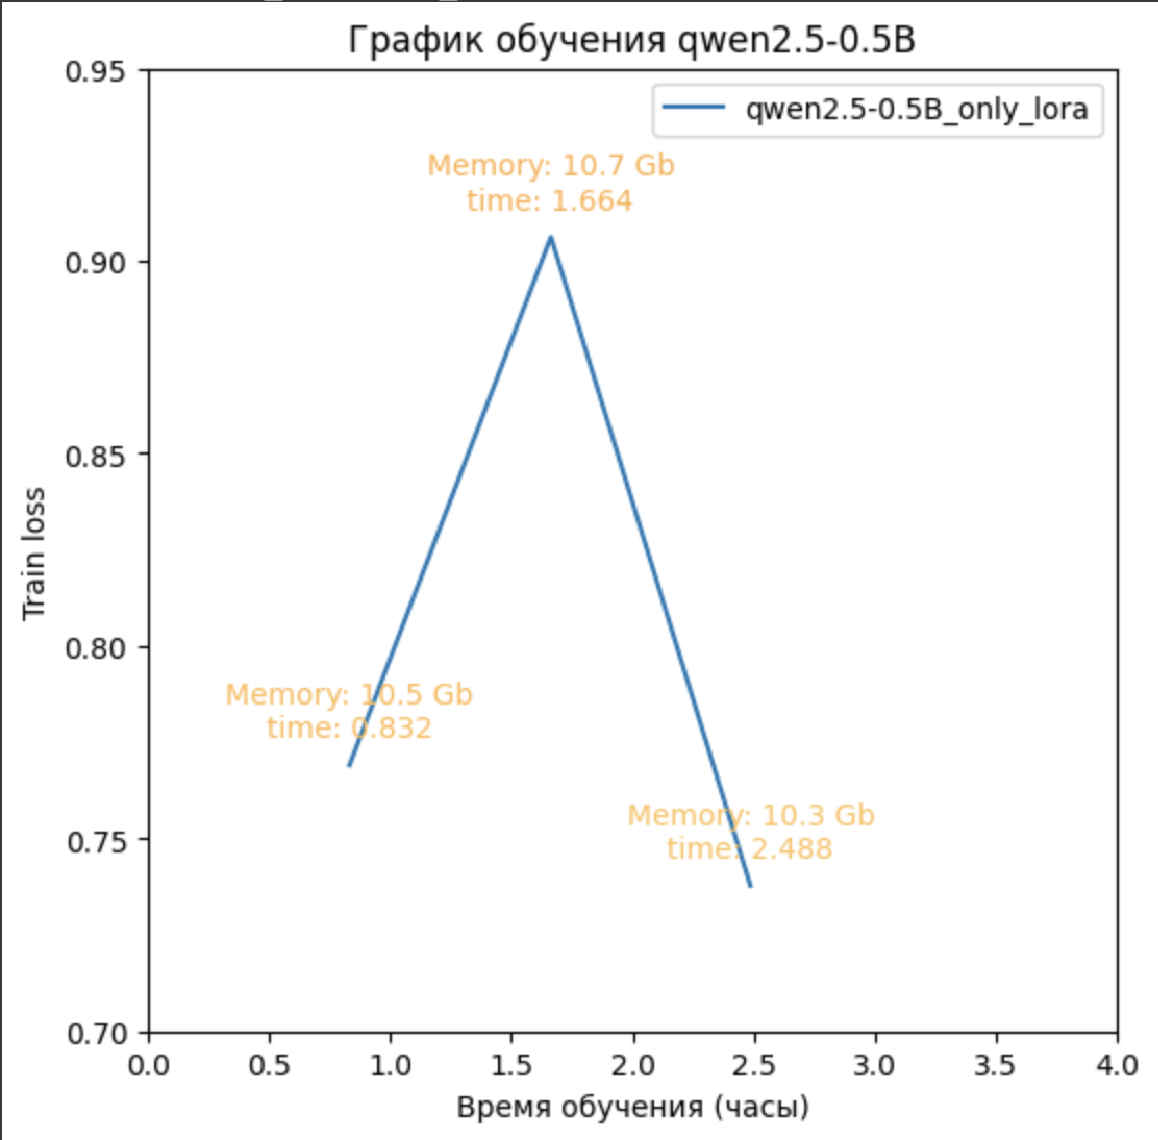
\includegraphics[scale=0.5]{images/qwen_training.pdf}

На графике изображено значение лосс функции во время обучения по эпохам

[Также вот таблица для будущей визуализации результатов]

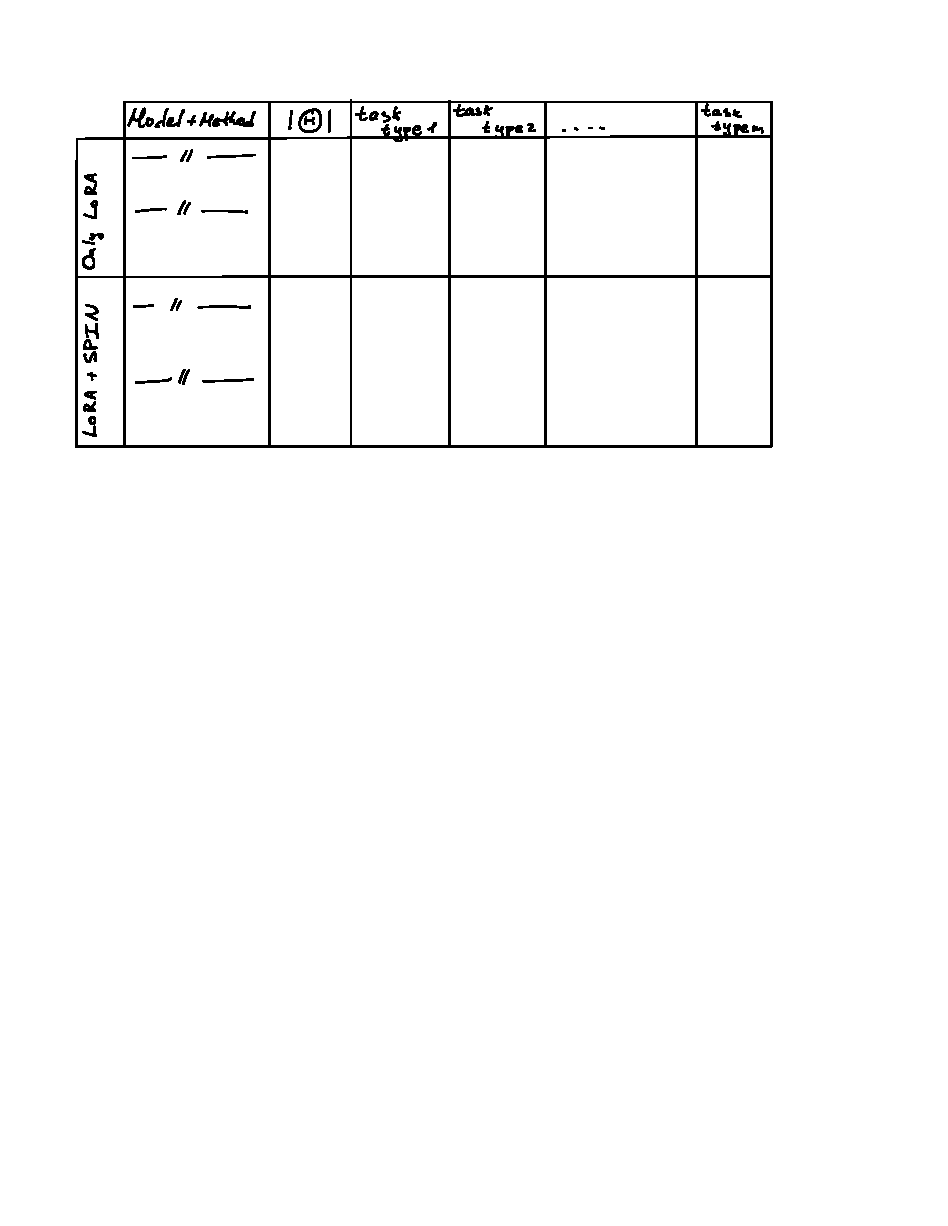
\includegraphics{images/table_draft.pdf}

Рассматриваются столбцы: модель + примененный метод дообучения, количество параметров, тип задачи (text generation, classification и т.д.) или датасеты, на котором происходит дообучения (не знаю что лучше использовать ). Слева изображены две графы, они будут убраны.

\printbibliography

\end{document}

